Experimental materials, unidentifiable-data, and R code are openly available through the Open Science Framework at: XXXX


\subsection{Participants}
A total of 128 participants were initially recruited for the study. Rather than use the term "native speaker" (see \cite{Brown_Tusmagambet_Rahming_Tu_DeSalvo_Wiener_2023} for a discussion on this term), we recruited participants according to their first language (L1), which we defined as the language acquired from birth and the language that the speaker considered most fluent. We defined the second language (L2) as the language acquired in childhood after the L1 was in place and the language that the speaker considers less fluent than their L1. The L1 English participants were recruited via Prolific (N = 25) or in-person at a North American university (N = 50). All L1 English participants reported being born in the United States. The L1 Dutch-L2 English speakers (N =53) were fully recruited via Prolific and all reported being born in the Netherlands. To ensure consistency, participants completed a detailed language background questionnaire \citep{Marian_Blumenfeld_Kaushanskaya_2007}, confirming their age of L2 acquisition, language exposure history, and self-rated proficiency. No participants had significant early exposure to other languages at home, and all participants completed primary and secondary education in English or Dutch-speaking environments, respectively. From these 128 participants, we required that all participants provide informed consent, pass a basic hearing screening using a dichotic pitch task \citep{milne_2021}, and pass a 5-point eye-tracking calibration with sufficient lighting. This left a total of 88 participants (L1 English N = 61; L1 Dutch N = 27) who qualified and completed the study. These participants were compensated for their time.

\subsection{Materials}
All materials used in the present study were freely available and taken from previously published research. The forward digit span task, Flanker task, and LexTALE \citep{lemhofer2012introducing} were taken from the Gorilla \citep{Anwyl-Irvine_2019} Open Materials repository (see our OSF for more details). The perceptual auditory sensitivity and auditory motor reproduction tasks were taken from \cite{Kachlicka_Saito_Tierney_2019, saito2020domain}. Auditory and visual stimuli for the eye-tracking task were provided by \cite{Ge2021}. Auditory stimuli were recorded at 44.1 kHz (16-bit resolution, mono) by a male native speaker of British English. 40 target sentences contained \textit{only} with prosodic prominence on either the verb or the object, creating two experimental conditions: object-focus and verb-focus. An additional 48 fillers were created without the \textit{only} focus particle. Like the targets, these fillers contained a \textit{not}-fragment as in "The rabbit is licking the CANDY, not licking the ice cream." Figure \ref{fig:sampleslide} shows an example of a 2x2 visual stimulus. Each stimulus consisted of a target (e.g., the rabbit licking the candy), a competitor corresponding to the alternative focus (e.g., the rabbit licking the ice cream), and two distractors (the rabbit throwing the candy, ice cream). The distractors were structured to ensure balanced looks across visual stimuli so that participants could not infer the target-competitor pairing by visual inspection alone.

\begin{figure}
    \centering
    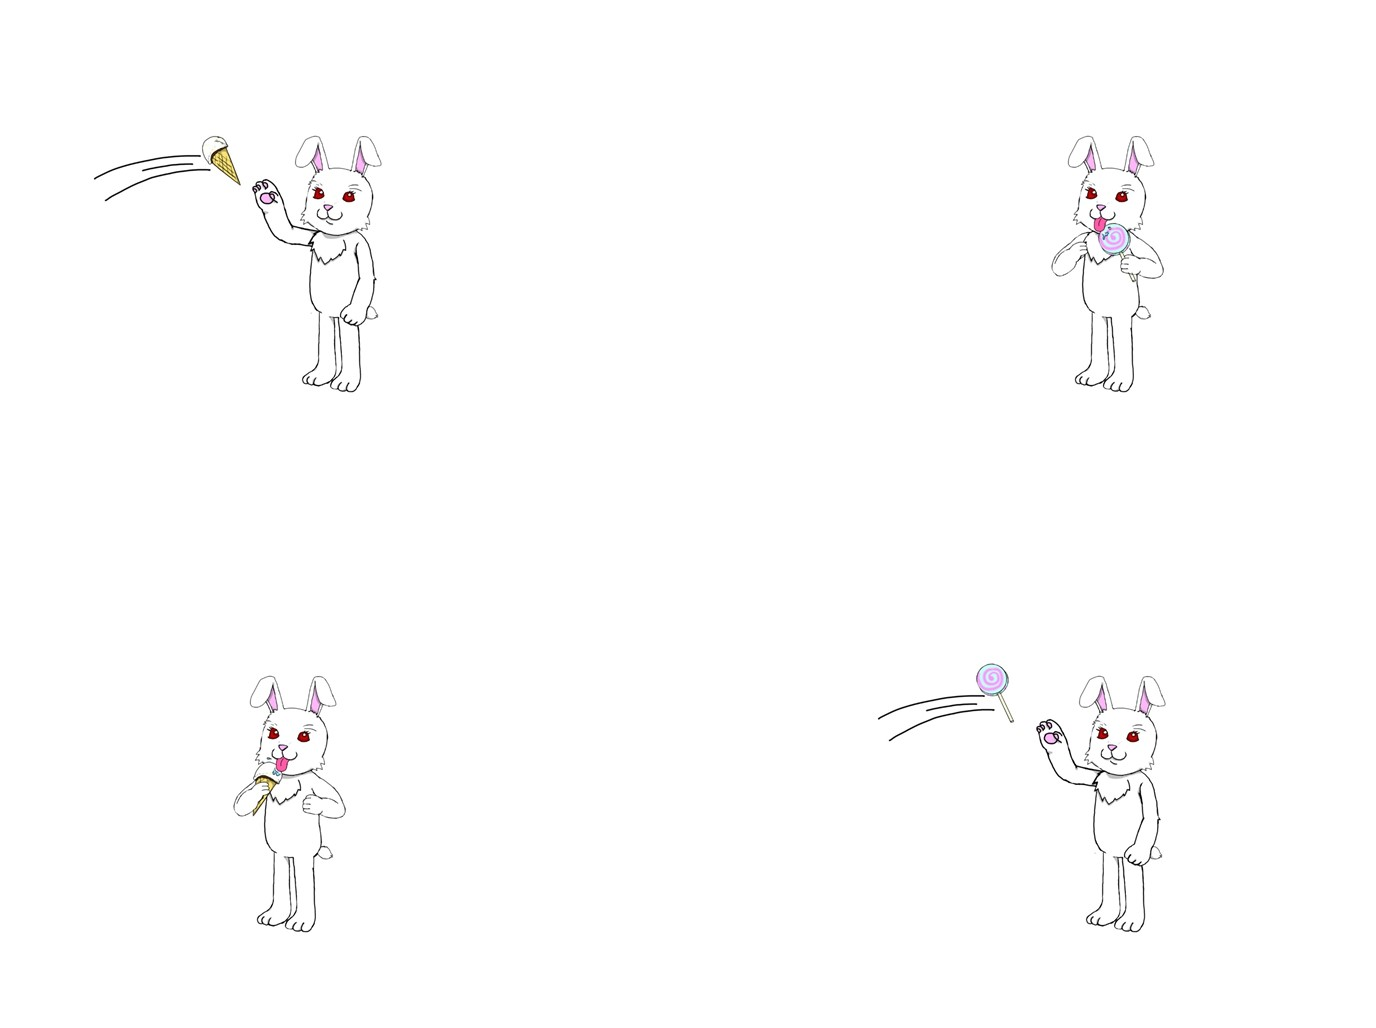
\includegraphics[width=\textwidth,height=\textheight,keepaspectratio]{viz/Fig1-Geetal.jpg}
    \caption{Example 2x2 visual display taken from Ge et al. (2021).}
    \label{fig:sampleslide}
\end{figure}


\subsection{Procedure}

The experiment was hosted on Gorilla \citep{Anwyl-Irvine_2019} and distributed via Prolific, with participants completing the study on a personal computer in an environment that met the experiment’s requirements, such as adequate lighting and minimal background noise. Only participants who consented and passed the hearing and eye-tracking calibration screenings proceeded to the main experiment.

Participants started with the first three tasks in a fixed order: digit span, auditory sensitivity, and Flanker. The digit span task began with two digits. Each digit appeared on screen for 500 ms, followed by a fixation cross for 250 ms. Participants were required to use their mouse and a visual number pad to enter the same digits in the same order. The adaptive, forward task increased by one digit after each correct response and decreased by one digit after each incorrect response. The task contained 13 trials and took approximately two minutes to complete. Cronbach's alpha for the task was .63. The auditory sensitivity task included four same/different (AX) discrimination tasks across four dimensions or cues:  pitch, risetime (the speed at which a sound reaches its peak amplitude), duration, and formant contrasts. The internal consistency of these tasks, measured by Cronbach’s alpha, was .75, .76, .60, .70, respectively. Each task consisted of 36 trials in which a sound was played, followed by a 250 ms fixation cross, and then a second sound. Participants responded by pressing the ‘z’ or ‘m’ key to indicate whether the sounds were the same or different. Each task used a continuum of 50 stimuli taken from \citep{Kachlicka_Saito_Tierney_2019}, with 10 stimuli selected at varying distances (15-55) (e.g., 10 Hz or 15 Hz for pitch). The order of stimulus distances and same/different trials was randomized. Each battery task took approximately 90 seconds to complete. We note that both the auditory sensitivity and digit span tasks contained items of varying difficulty. For example, recalling two digits is inherently easier than recalling nine digits; discriminating between two sounds with a 50 Hz difference is easier than discriminating between two sounds with a 5 Hz difference. Given this variability, lower internal reliability, as measured by \cite{Cronbach1951}, is expected. These results mirror the findings of \cite{ppcc}.

Next, participants either took part in the main eye-tracking task or the auditory-motor tasks. The eye-tracking task and the auditory-motor tasks were counterbalanced across participants to mitigate order effects and minimize potential biases related to task sequencing.

For the eye-tracking task, gaze data were recorded using WebGazer.js \citep{Papoutsaki}, implemented within Gorilla \citep{Anwyl-Irvine_2019}. 

The primary task (2×2 visual world paradigm design) consisted of 40 English sentences with preverbal only, adapted from \cite{Ge_etal_2021}, with an additional 48 filler items. The original auditory stimuli were recorded at 44.1 kHz (16-bit resolution, mono) by a male native speaker of British English.

Participants completed 128 trials, during which 64 experimental and distractor words were presented in lowercase letters (font size 20) and evenly distributed across four quadrants to maximize spatial separation between areas of interest \citep{bramlett_wiener_24-AOW}. The presentation order of experimental and distractor trials was randomized. Each trial followed the procedure outlined in \cite{Ge_et_al}, beginning with a 500 ms fixation cross, after which the audio and visual stimuli were presented concurrently alongside the carrier phrase “Clicca sulla parola” (‘click on the word’). Once the audio file finished playing ($\mu$ = 1819 ms, $\sigma$ = 101 ms), the visual stimuli remained on-screen for 5000 ms or until the participant selected a response. The task was preceded by a practice session to ensure that participants were familiar with the procedure. Unlike \cite{Ge_et_al}, who included a read-aloud familiarization task, this study omitted that step. Their findings indicated that all participants were already familiar with the stimuli, and prior norming data confirmed that no participants were unfamiliar with the words. The removal of this component also shortened the overall duration of the experiment. The eye-tracking task took approximately seven minutes to complete.

The auditory-motor tasks consisted of two components: auditory-motor rhythm and auditory-motor melody, both adapted from \citep{Kachlicka_Saito_Tierney_2019}. In the auditory-motor rhythm task, participants heard a rhythmic sequence consisting of 13 possible beat positions, played three times. They were then required to replicate the rhythm by pressing the space bar at the correct intervals. Each key press was time-stamped to assess accuracy. In the auditory-motor melody task, participants listened to a seven-note melody and were required to reproduce it using on-screen buttons corresponding to relative pitch levels. To maintain consistency, all melodies began with the middle pitch, ensuring a stable reference point for participants.

Lastly, After completing the eye-tracking task and audio-motor tasks, participants proceeded to a modified version of the English LexTALE task \citep{lemhofer2012introducing}. These tasks were deliberately placed after the eye-tracking task to minimize any potential interference with task performance. In the English LexTALE task, participants first saw a 500 ms fixation cross followed by a string of letters presented for 2000 ms. Participants used the 'j' and 'k' keys to indicate whether the displayed string was a real word or a non-word, within the given time limit \citep{lemhofer2012introducing}. A total of 60 trials were completed, consisting of 40 words and 20 non-words, and this task took approximately three minutes to complete. The internal consistency for the LexTALE task, measured by Cronbach’s alpha, was x. The English LexTALE and was adapted from publicly available Gorilla open materials; while the original versions of LexTALE did not impose time limits, our version required responses within 2000 ms.

Additionally, participants completed a language experience questionnaire designed to assess their language background and experience. This questionnaire was used to ensure that participants had the appropriate language experience for the study.

\subsubsection{Data analysis}

